Emergence and rapid advancements in multicore CPUs have driven substantial acceptance of shared memory parallel computing platforms. CPUs offer parallel computing platforms at laptop, desktop, and server levels, making them ubiquitous and exposing performance almost everywhere. The most common form of CPU architecture is cache-coherent Non-Uniform Memory Access (cc-NUMA), which is characterized by access times not being completely uniform. Even many small dual-socket general-purpose CPU systems have this kind of memory system. This architecture has become dominant because the number of cores in a processor, as well as the number of sockets, continues to increase.\par

In a cc-NUMA CPU system, each socket connects to a subset of the total memory in the system. A cache-coherent interconnect glues all of the sockets together and provides a single system view for programmers. Such a memory system is scalable, because the aggregate memory bandwidth scales with the number of sockets in the system. The benefit of the interconnect is that an application has transparent access to all of the memory in the system, regardless of where the data resides. However, there is a cost: the latency to access data and instructions, from memory is no longer consistent (e.g., fixed access latency). The latency instead depends on where that data is stored in the system. In a good case, data comes from memory directly connected to the socket where code runs. In a bad case, data has to come from a memory connected to a socket far away in the system, and that cost of memory access can increase due to the number of hops in the interconnect between sockets on a cc-NUMA CPU system.\par

In Figure 16-1, a generic CPU architecture with cc-NUMA memory is shown. This is a simplified system architecture containing cores and memory components found in contemporary, general-purpose, multisocket systems today. Throughout the remainder of this chapter, the figure will be used to illustrate the mapping of corresponding code examples.\par

To achieve optimal performance, we need to be sure to understand the characteristics of the cc-NUMA configuration of a specific system. For example, recent servers from Intel make use of a mesh interconnect architecture. In this configuration, the cores, caches, and memory controllers are organized into rows and columns. Understanding the connectivity of processors with memory can be critical when working to achieve peak performance of the system.\par

\hspace*{\fill} \par %插入空行
Figure 16-1. Generic multicore CPU system
\begin{center}
	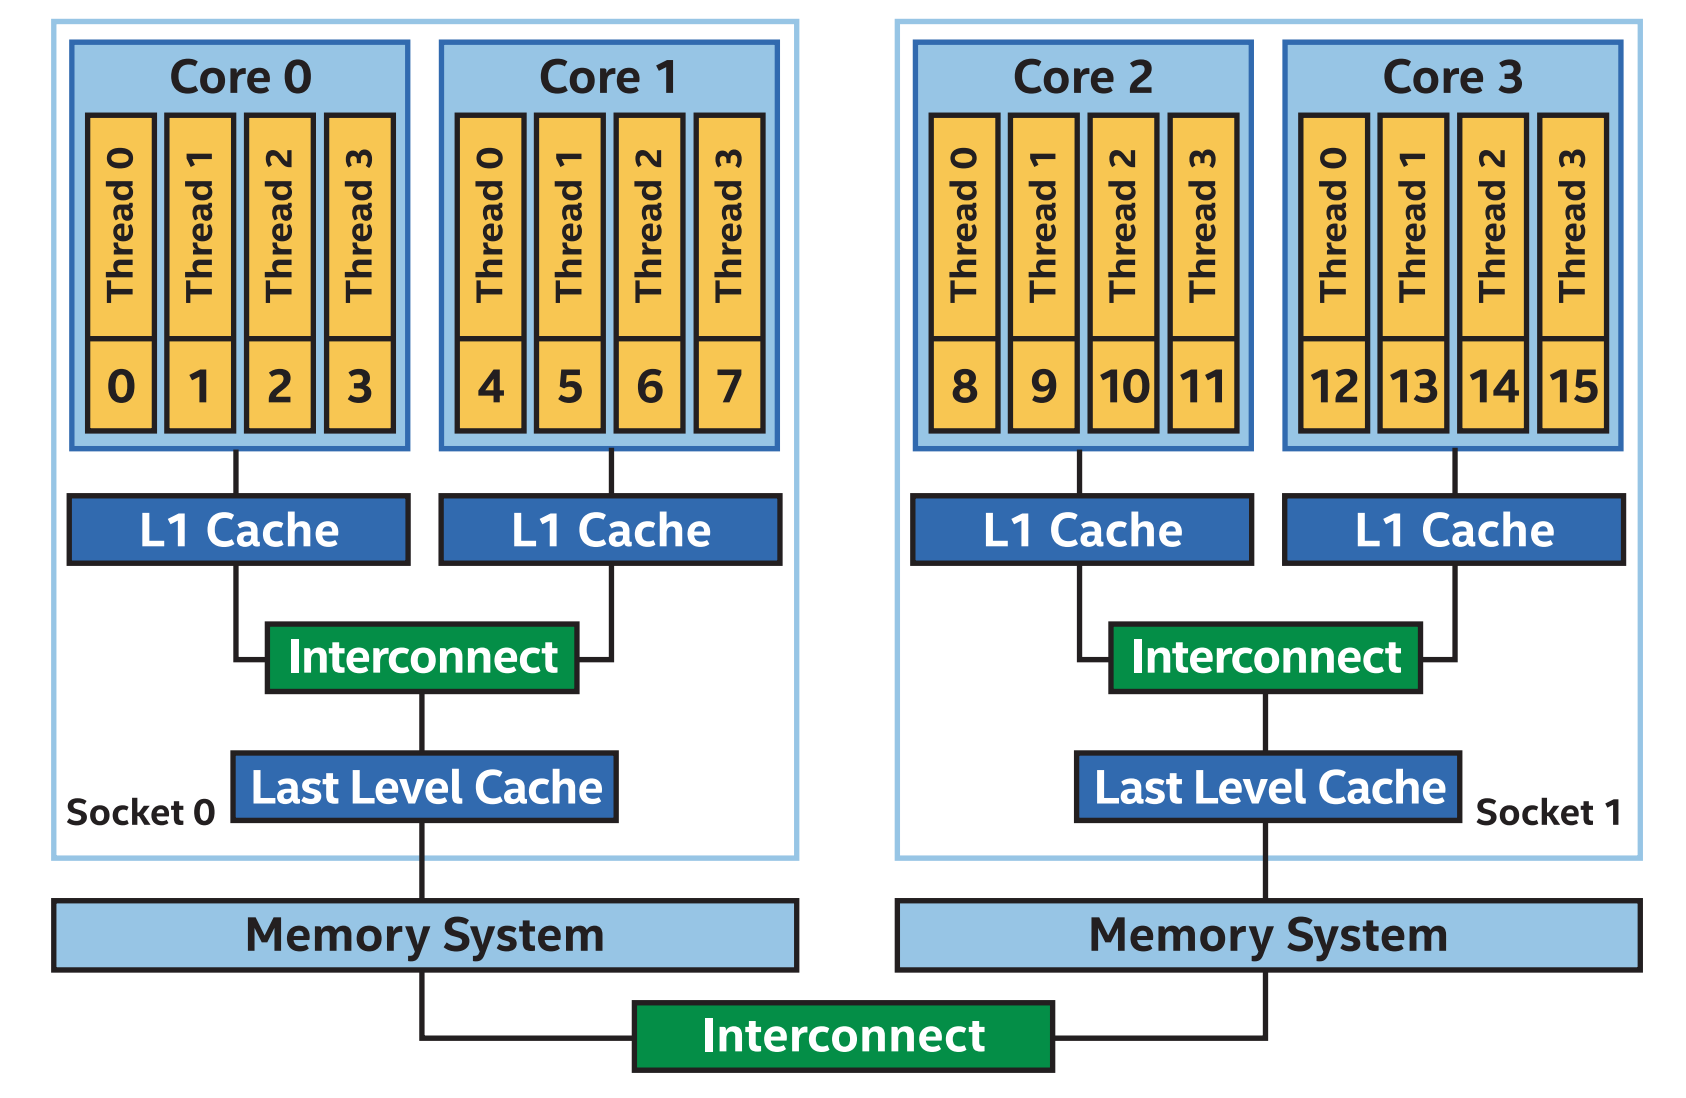
\includegraphics[width=1.0\textwidth]{content/chapter-16/images/2}
\end{center}

The system in Figure 16-1 has two sockets, each of which has two cores with four hardware threads per core. Each core has its own level 1 (L1) cache. L1 caches are connected to a shared last-level cache, which is connected to the memory system on the socket. The memory access latency within a socket is uniform, meaning that it is consistent and can be predicted with accuracy.\par

The two sockets are connected through a cache-coherent interconnect. Memory is distributed across the system, but all of the memory may be transparently accessed from anywhere in the system. The memory read and write latency is non-uniform when accessing memory that isn’t in the socket where code making the access is running, which means it imposes a potentially much longer and inconsistent latency when accessing data from a remote socket. A critical aspect of the interconnect, though, is coherency. We do not need to worry about data becoming inconsistent across the memory system (which would be a functional problem) and instead need to worry only about the performance impact of how we’re accessing the distributed memory system.\par

Hardware threads in CPUs are the execution vehicles. These are the units that execute instruction streams (a thread in CPU terminology). The hardware threads in Figure 16-1 are numbered consecutively from 0 to 15, which is a notation used to simplify discussions on the examples in this chapter. Unless otherwise noted, all references to a CPU system in this chapter are to the reference cc-NUMA system shown in Figure 16-1.\par




























































